%%%% Header %%%%%%%%%%%%%%%%%%%%%%%%%%%%%%%%%%%%%%%%%%%%%%%%%%%%%%%%%%%%%%%%%%%

\documentclass{beamer}

%%%% Packages %%%%%%%%%%%%%%%%%%%%%%%%%%%%%%%%%%%%%%%%%%%%%%%%%%%%%%%%%%%%%%%%%

% font/encoding
\usepackage[utf8]{inputenc} % .tex-file text encoding
\usepackage[T1]{fontenc} % vector fonts and hiQual special chars in output
\usepackage{libertine} % libertine font family
\usepackage[libertine]{newtxmath} % libertine mathematics
\usepackage[scaled=0.85]{inconsolata} % monospace font

% localization
\usepackage[english]{babel} % document language/localization

% maths
\usepackage{amsmath} % various maths features
\usepackage{mathtools} % aligned matrices

% figures
\usepackage{graphicx} % include external images
\usepackage[compatibility=false]{caption} % figure captions
\usepackage{subcaption} % captions for subfigures

% verbatim
\usepackage{listings} % source code environment

% tables
\usepackage{booktabs} % nice table rules
\usepackage{dcolumn} % column alignment at decimal point

% bibliography
\usepackage[style = authoryear-ibid, % bibliography using biblatex
            backend = biber,
            bibencoding = utf8,
            doi = false,
            isbn = false]{biblatex}

%%%% General layout %%%%%%%%%%%%%%%%%%%%%%%%%%%%%%%%%%%%%%%%%%%%%%%%%%%%%%%%%%%

% colours
\definecolor{maincol}{RGB}{46, 69, 136} % main deco colour
\usecolortheme{dove} % black/grey colours
% font
\usefonttheme{serif} % use serif fonts
\setbeamerfont{frametitle}{series=\bfseries}
% inner theme
\useinnertheme{rectangles}
% header
\useoutertheme{miniframes} % nice shading in header
\setbeamertemplate{headline}{} % disable section tree
\setbeamercolor{frametitle}{fg=white, bg=maincol}
% footline
\setbeamertemplate{navigation symbols}{} % no nav symbols
\setbeamertemplate{footline}[page number] % page number
% figures
\setkeys{Gin}{width=1.0\textwidth} % figures fill textwidth
\setbeamertemplate{caption}{\insertcaption} % no caption label
\setbeamertemplate{caption label separator}{}
% list
\setbeamertemplate{itemize items}[triangle] % list symbol
% bibliography
\setbeamertemplate{bibliography item}{} % no bibliography icon
% pdf
\hypersetup{pdfstartview={Fit}} % fit the presentation to the window
% box colours
\setbeamercolor*{block title}{fg=white,bg=darkgray}
\setbeamercolor*{block body}{fg=black, bg=lightgray}

%%%% Special layout %%%%%%%%%%%%%%%%%%%%%%%%%%%%%%%%%%%%%%%%%%%%%%%%%%%%%%%%%%%

% figure placeholder (comment out to disable)
% \makeatletter
%   \AtBeginDocument{%
%     \def\Ginclude@graphics#1{%
%       \begingroup\fboxsep=-\fboxrule
%       \fbox{\rule{\@ifundefined{Gin@@ewidth}{150pt}{\Gin@@ewidth}}{0pt}%
%         \rule{0pt}{\@ifundefined{Gin@@eheight}{100pt}{\Gin@@eheight}}}\endgroup}}
% \makeatother

%%%% Tables %%%%%%%%%%%%%%%%%%%%%%%%%%%%%%%%%%%%%%%%%%%%%%%%%%%%%%%%%%%%%%%%%%%

% global table format
\newcommand{\tabformat}{\small\centering}
% fontsize of table footnote
\newcommand{\tabfontsizefoot}{\footnotesize}
% dcolumn column type
\newcolumntype{d}{D{,}{,}}
% centering with fixed column size in tables
\newcolumntype{Q}[1]{>{\centering\arraybackslash}p{#1}}
% raggedright in tables
\newcolumntype{P}[1]{>{\raggedright\hspace{0pt}\arraybackslash}p{#1}}
% no space between table columns
\renewcommand{\tabcolsep}{0cm}

%%%% Listings %%%%%%%%%%%%%%%%%%%%%%%%%%%%%%%%%%%%%%%%%%%%%%%%%%%%%%%%%%%%%%%%%

% help package "listings" to represent german special chars
\lstset{literate=%
{Ö}{{\"O}}1
{Ä}{{\"A}}1
{Ü}{{\"U}}1
{ß}{{\ss}}1
{ü}{{\"u}}1
{ä}{{\"a}}1
{ö}{{\"o}}1
}

\lstset{
language = R,
% sets automatic line breaking
breaklines = true,
% where to put the line-numbers; possible values are (none, left, right)
numbers = left,
% how far the line-numbers are from the code
numbersep = 5pt,
% the style that is used for the line-numbers
numberstyle = \tiny,
% the step between two line-numbers. If it's 1, each line will be numbered
stepnumber = 1,
% font and size for code
basicstyle = \ttfamily\footnotesize,
% mark linebreaks
prebreak = \raisebox{0ex}[0ex][0ex]{\ensuremath{\rhookswarrow}},
postbreak=\raisebox{0ex}[0ex][0ex]{\ensuremath{\rcurvearrowse\space}},
% colors
commentstyle=\color{maincol}
}

%%%% Paths %%%%%%%%%%%%%%%%%%%%%%%%%%%%%%%%%%%%%%%%%%%%%%%%%%%%%%%%%%%%%%%%%%%%

% figures
\graphicspath{{/home/jon/lucile/share/hive/sci/infrail/talk/2015-02-02-odense-infrail/fig/}}

% bibliography file
\bibliography{/home/jon/lucile/bibliothek/bibtex/bibliography.bib}

%%%% meta data %%%%%%%%%%%%%%%%%%%%%%%%%%%%%%%%%%%%%%%%%%%%%%%%%%%%%%%%%%%%%%%%

\title{Human Early Life Mortality}
\subtitle{Adaption or Selection?}
\author{Jonas Schöley\\\url{schoeley@demogr.mpg.de}}
\institute{
\includegraphics[width = 3cm]{./EDSDLogo.pdf}}
\subject{Human Early Life Mortality}
\keywords{infant mortality, childhood mortality, frailty, selection, adaption, heterogeneity}

%%%% titlepage %%%%%%%%%%%%%%%%%%%%%%%%%%%%%%%%%%%%%%%%%%%%%%%%%%%%%%%%%%%%%%%%

\setbeamerfont{title}{size=\LARGE, series=\bfseries}
\setbeamerfont{subtitle}{size=\Large, series=\mdseries}
\setbeamerfont{author}{size = \normalsize, series=\mdseries}
\setbeamerfont{institute}{size=\normalsize, series=\mdseries}
\defbeamertemplate*{title page}{customized}[1][]
{
  \centering
  \usebeamerfont{title}\inserttitle\\\medskip
  \usebeamerfont{subtitle}\usebeamercolor[fg]{subtitle}\insertsubtitle\par
  \vfill
  \usebeamerfont{author}\insertauthor\par
  \vfill
  \usebeamerfont{institute}\insertinstitute\par
  \usebeamercolor[fg]{titlegraphic}\inserttitlegraphic
}

\begin{document}

{
\usebackgroundtemplate{
\includegraphics[width=\paperwidth]{./fig/background.png}}%
\begin{frame}[plain]
\titlepage
\end{frame}
}

\section{The Age Pattern of Early Life Mortality} %%%%%%%%%%%%%%%%%%%%%%%%%%%%%

%\usebackgroundtemplate{\includegraphics[width=\paperwidth]{./misc/background2.png}}

\begin{frame}
\frametitle{\insertsection}

\begin{columns}[c]

\column{0.75\textwidth}
\begin{figure}[htb!]
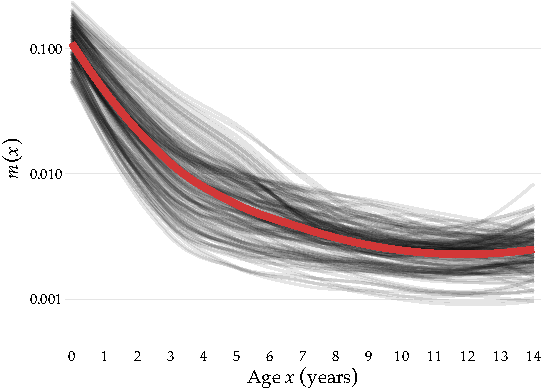
\includegraphics[width = \textwidth]{./plot-hmd_mx.pdf}\\
\end{figure}

\column{0.25\textwidth}
\footnotesize\textbf{Early life mortality rates}\\ Various countries and years.\\ \scriptsize\emph{Data: HMD.}

\end{columns}

\end{frame}

\section{Adaption Models of Early Life Mortality} %%%%%%%%%%%%%%%%%%%%%%%%%%%%%

\begin{frame}
\frametitle{\insertsection}

\begin{columns}[c]

\column{0.5\textwidth}
\begin{equation*}
m(x) = A^{(x + B)^C}
\end{equation*}

\bigskip

\begin{equation*}
m(x) = ae^{-bx}
\end{equation*}

\column{0.5\textwidth}
\footnotesize\textbf{\citeauthor{Heligman1980} infant mortality term}\\ Double exponential distribution. \\
\emph{\enquote{$C$ measures the rate of mortality decline in childhood (the rate at which a child adapts to its environment).}} \\ \scriptsize\emph{\cite{Heligman1980}.}

\medskip

\footnotesize\textbf{\citeauthor{Siler1979} infant mortality term}\\ Negative-$b$-Gompertz hazard. \\
\emph{\enquote{While the most common use of this decreasing hazard would be to account for the hazard due to immaturity, it can also be used [$\ldots$] for other hazards to which an animal adjusts successfully.}}
\\ \scriptsize\emph{\cite{Siler1979}.}

\end{columns}

\end{frame}

%

\begin{frame}
\frametitle{\insertsection}

\begin{columns}[c]

\column{0.65\textwidth}
\begin{figure}[htb!]
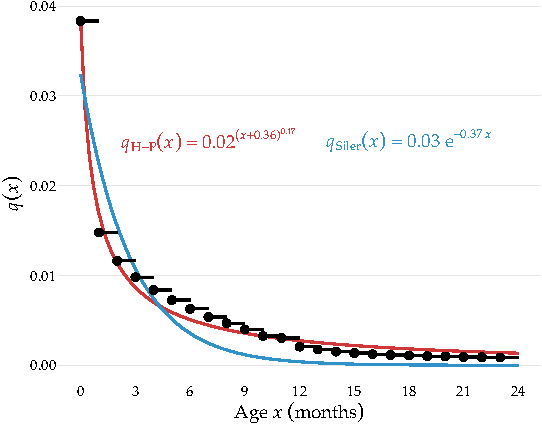
\includegraphics[width = \textwidth]{./plot-adaptive.pdf}\\
\end{figure}

\column{0.35\textwidth}
\footnotesize\textbf{Adaption models of infant mortality}\\ Observed versus predicted probabilities of dying. \cite{Heligman1980} and \cite{Siler1979} model infant mortality terms. \\ \scriptsize\emph{Data: \cite{Danmark1920}. 1911--1915 period of Danish males.}

\end{columns}

\end{frame}

\section{Mechanisms of Adaption} %%%%%%%%%%%%%%%%%%%%%%%%%%%%%%%%%%%%%%%%%%%%%%

\begin{frame}
\frametitle{\insertsection}

\begin{figure}[htb!]
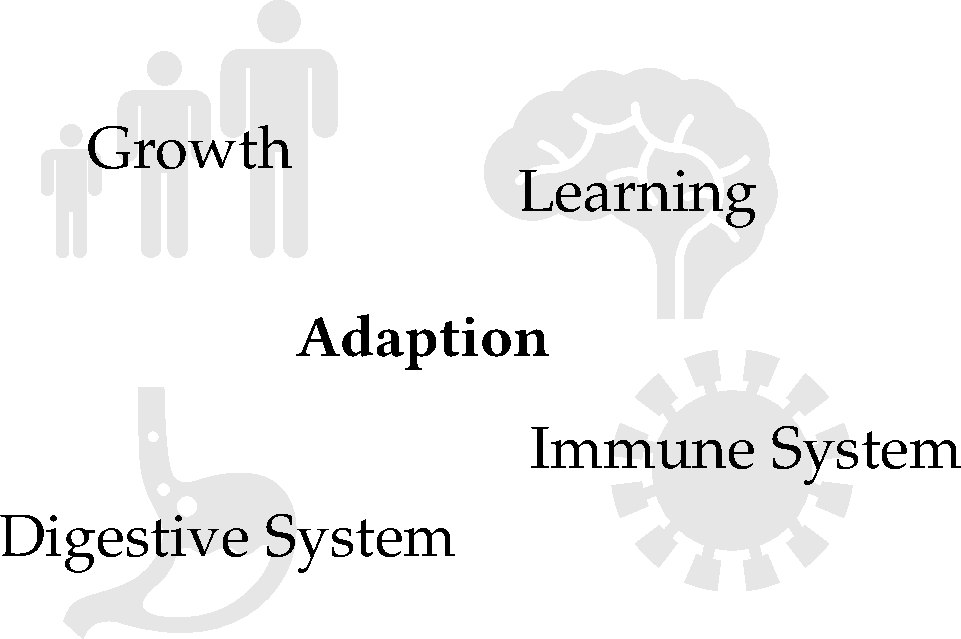
\includegraphics[width = 0.8\textwidth]{./adaption.pdf}\\
\end{figure}

\end{frame}

\section{A Selection Model of Early Life Mortality} %%%%%%%%%%%%%%%%%%%%%%%%%%%

\begin{frame}
\frametitle{\insertsection}

\begin{columns}[c]

\column{0.65\textwidth}
\begin{figure}[htb!]
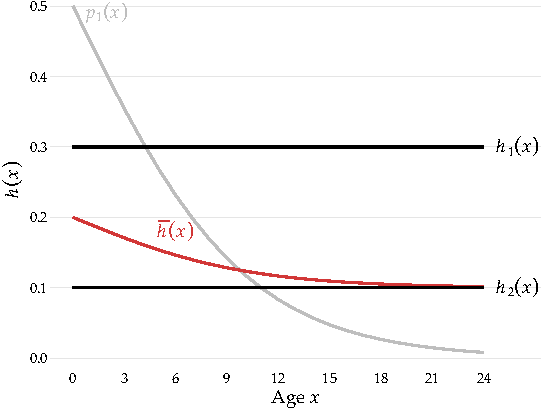
\includegraphics[width = \textwidth]{./plot-binary.pdf}\\
\end{figure}

\column{0.35\textwidth}
\footnotesize\textbf{The selection effect of heterogeneous mortality}\\
$h_{1,2}(x)$: Baseline mortality rates for two groups.\\
$\bar{h}(x)$: Population mortality rate.\\
$p_1(x)$: Share of group 1 on the total population. \\ \scriptsize\emph{See \cite{Vaupel1985} for more of \enquote{Heterogeneity's Ruses}.}

\end{columns}

\end{frame}

\begin{frame}
\frametitle{\insertsection}

\textbf{The Frailty Model:} \fullcite{Vaupel1979}

\vfill

\begin{columns}[c]

\column{0.5\textwidth}
\begin{equation*}
\mu(x|z) = \underbrace{z}_{\substack{\text{Frailty}}} \cdot \underbrace{\mu_0(x)}_{\substack{\text{Baseline} \\ \text{hazard}}}
\end{equation*}

\medskip

\begin{equation*}
\bar{\mu}(x) = \frac {\mu_0(x)} {\gamma M_0(x) + 1}
\end{equation*}

\column{0.5\textwidth}
\footnotesize\textbf{Individual hazard with frailty}\\ Mortality at $x$ for single individual with given frailty factor $z$. \\ \scriptsize\emph{\cite{Vaupel1979}.}

\medskip

\footnotesize\textbf{Mean population hazard with frailty}\\ Mean mortality in population at $x$ \\ \scriptsize\emph{\cite{Vaupel1979}.}

\end{columns}

\end{frame}

%

\begin{frame}
\frametitle{\insertsection}

\begin{columns}[c]

\column{0.65\textwidth}
\begin{figure}[htb!]
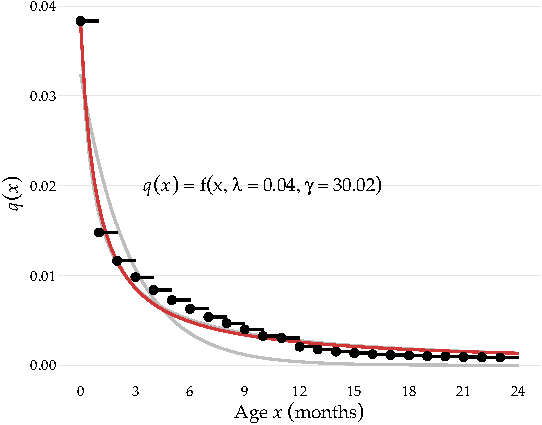
\includegraphics[width = \textwidth]{./plot-selective.pdf}\\
\end{figure}

\column{0.35\textwidth}
\footnotesize\textbf{A selective model of infant mortality}\\ Observed versus predicted probabilities of dying. Exponential-Gamma frailty model. \\ \scriptsize\emph{Data: \cite{Danmark1920}. 1911--1915 period of Danish males.}

\end{columns}

\end{frame}

\section{References} %%%%%%%%%%%%%%%%%%%%%%%%%%%%%%%%%%%%%%%%%%%%%%%%%%%%%%%%%%

\begin{frame}
\frametitle{\insertsection}

\nocite{Hmd2015}

\printbibliography

\end{frame}

\end{document}